\documentclass[11pt,a4paper]{article}
\usepackage[margin=20mm,headheight=15pt]{geometry}
\usepackage{fontspec}
\setmainfont{Liberation Sans}
\setmonofont{Liberation Mono}[Scale=0.86]
\usepackage{amsmath,amssymb,array,booktabs,tabularx,longtable}
\usepackage[table]{xcolor}
\usepackage{graphicx,tikz}
\usetikzlibrary{arrows.meta,positioning,fit,calc,backgrounds}
\usepackage{listings,fancyhdr,titlesec,caption,xurl}
\usepackage[colorlinks=true,linkcolor=teal,urlcolor=teal,citecolor=teal]{hyperref}
\definecolor{navy}{HTML}{16324F}
\definecolor{teal}{HTML}{087F8C}
\definecolor{pale}{HTML}{EAF4F5}
\definecolor{graybg}{HTML}{F3F5F7}
\definecolor{muted}{HTML}{4D5D6C}
\definecolor{amber}{HTML}{936018}
\hypersetup{pdftitle={Monitor de aire con ESP32-S3: reporte de practica IoT},pdfauthor={Proyecto MonitorAire},pdfsubject={Sensores, MQTT, persistencia CSV y conversion modular Python}}
\renewcommand{\contentsname}{Contenido}
\renewcommand{\figurename}{Figura}
\renewcommand{\tablename}{Tabla}
\renewcommand{\refname}{Referencias técnicas}
\titleformat{\section}{\Large\bfseries\color{navy}}{\thesection.}{0.5em}{}
\titleformat{\subsection}{\normalsize\bfseries\color{teal}}{\thesubsection}{0.5em}{}
\titlespacing*{\section}{0pt}{3mm}{3mm}
\titlespacing*{\subsection}{0pt}{3mm}{1.5mm}
\setlength{\parindent}{0pt}
\setlength{\parskip}{5pt}
\setlength{\tabcolsep}{5pt}
\renewcommand{\arraystretch}{1.22}
\setcounter{tocdepth}{1}
\pagestyle{fancy}
\fancyhf{}
\fancyhead[L]{\small\color{muted}MonitorAire · ESP32-S3}
\fancyhead[R]{\small\color{muted}Reporte de práctica IoT}
\fancyfoot[L]{\small\color{muted}Código, implementación y resultados}
\fancyfoot[R]{\small\thepage}
\renewcommand{\headrulewidth}{0.3pt}
\lstset{basicstyle=\ttfamily\footnotesize,breaklines=true,columns=fullflexible,keepspaces=true,showstringspaces=false,frame=single,rulecolor=\color{gray!25},backgroundcolor=\color{graybg},framesep=6pt,aboveskip=7pt,belowskip=6pt,tabsize=4}
\newcolumntype{P}[1]{>{\raggedright\arraybackslash}p{#1}}
\newcolumntype{Y}{>{\raggedright\arraybackslash}X}
\urlstyle{tt}
\newcommand{\code}[1]{\expandafter\nolinkurl\expandafter{\detokenize{#1}}}
\setlength{\emergencystretch}{2em}
\newcommand{\note}[1]{\par\smallskip\noindent\colorbox{pale}{\parbox{\dimexpr\linewidth-14pt\relax}{\small\textbf{Criterio de interpretación.} #1}}\par\smallskip}
\newcommand{\nextsection}[1]{\clearpage\section{#1}}

% Diagramas con tarjetas, corredores reservados y tipografia de ancho fijo.
\definecolor{bluepale}{HTML}{EEF3FA}
\definecolor{warmpale}{HTML}{FCF3E6}
\definecolor{linegray}{HTML}{D4DEE7}
\tikzset{
  card/.style={draw=linegray,fill=graybg,rounded corners=2.5mm,
    line width=.65pt,align=center,font=\fontsize{9.5}{12}\selectfont,
    text=navy,text width=42mm,inner xsep=3mm,inner ysep=3mm,minimum height=22mm},
  compute/.style={card,draw=navy!35,fill=bluepale},
  network/.style={card,draw=teal!55,fill=pale},
  storage/.style={card,draw=amber!45,fill=warmpale},
  strong/.style={card,draw=navy,fill=navy,text=white},
  chip/.style={align=center,text width=44mm,font=\fontsize{8}{10}\selectfont\bfseries,
    text=muted,inner sep=1mm},
  flow/.style={-{Stealth[length=2mm,width=1.5mm]},line width=.9pt,draw=teal,
    rounded corners=1.5mm},
  ackflow/.style={-{Stealth[length=2mm,width=1.5mm]},line width=.9pt,
    draw=amber,dashed,rounded corners=1.5mm},
  groupbox/.style={draw=linegray,fill=graybg!55,rounded corners=3mm,line width=.6pt},
  grouptitle/.style={anchor=west,font=\fontsize{8}{10}\selectfont\bfseries,
    text=muted,inner sep=0pt},
  participant/.style={card,text width=42mm,minimum height=15mm,inner ysep=2mm},
  message/.style={align=center,text width=54mm,fill=white,
    font=\fontsize{8.5}{10}\selectfont,text=navy,inner sep=1mm},
  activity/.style={draw=teal!40,fill=pale,rounded corners=2mm,text=navy,
    font=\fontsize{8.5}{10}\selectfont,align=center,text width=40mm,
    inner sep=2mm,minimum height=12mm}
}

\begin{document}
\begin{titlepage}
\thispagestyle{empty}
\vspace*{13mm}
{\color{teal}\large REPORTE TÉCNICO DE PRÁCTICA}\par
\vspace{8mm}
{\color{navy}\fontsize{32}{37}\selectfont\bfseries Monitor de aire\par con ESP32-S3}\par
\vspace{6mm}
{\Large Sensores, visualización local y comunicación MQTT}\par
\vspace{8mm}
{\large Persistencia en CSV y procesamiento modular en Python}\par
\vspace{14mm}
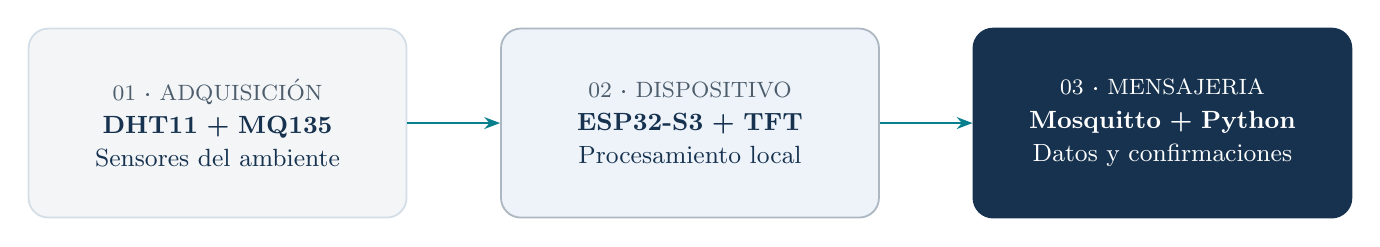
\begin{tikzpicture}[x=1mm,y=1mm]
\node[card,text width=42mm,minimum height=24mm] (a) at (25,0)
  {\textcolor{muted}{\footnotesize 01 · ADQUISICIÓN}\\\textbf{DHT11 + MQ135}\\Sensores del ambiente};
\node[compute,text width=42mm,minimum height=24mm] (b) at (85,0)
  {\textcolor{muted}{\footnotesize 02 · DISPOSITIVO}\\\textbf{ESP32-S3 + TFT}\\Procesamiento local};
\node[strong,text width=42mm,minimum height=24mm] (c) at (145,0)
  {{\footnotesize 03 · MENSAJERIA}\\\textbf{Mosquitto + Python}\\Datos y confirmaciones};
\draw[flow] (a)--(b);\draw[flow] (b)--(c);
\end{tikzpicture}
\vfill
\begin{tabularx}{\linewidth}{@{}lY@{}}
\textbf{Proyecto} & MonitorAire \\
\textbf{Dispositivo de ejemplo} & \code{ESP32_S3_0001} \\
\textbf{Plataforma} & PlatformIO, framework Arduino, ESP32-S3-DevKitC-1 \\
\textbf{Fecha del reporte} & 9 de noviembre de 2026 \\
\textbf{Base de análisis} & Código del proyecto y evidencias compartidas durante la práctica \\
\end{tabularx}
\vspace{7mm}
{\color{muted}\small Documento académico y técnico. Las cifras de gas son estimaciones del modelo implementado; no equivalen a una medición certificada de CO\textsubscript{2}.}
\end{titlepage}

\section*{Resumen}
\addcontentsline{toc}{section}{Resumen}
Se desarrolló un sistema de monitoreo ambiental con un ESP32-S3, un sensor DHT11 para temperatura y humedad, un módulo MQ135 para una estimación de gas y una pantalla ST7789 de 240\,$\times$\,320 píxeles. El firmware toma muestras aproximadamente cada dos segundos, presenta la información localmente y publica un documento JSON mediante MQTT cuando existe conexión con el broker.

Para conservar lecturas durante una interrupción se implementó un único archivo \code{/pending.csv} en LittleFS. Al reconectar, el dispositivo envía una fila por mensaje a un topic de datos crudos. Un programa Python modular valida esa fila, genera el mismo esquema JSON y lo publica en el topic tratado. Solo después de confirmar esta publicación con el broker envía el ID del registro al ESP32. El dispositivo guarda su avance en NVS y elimina el archivo cuando todas sus filas están confirmadas.

Las evidencias muestran comunicación entre ESP32, Mosquitto, Python y un suscriptor de terminal; recuperación de lecturas históricas; sincronización de fecha; y valores válidos de temperatura, humedad y gas estimado. También se documentan límites: publicaciones actuales con QoS 0, posibles duplicados, referencia de gas no contrastada y destello blanco de la pantalla aún sin causa confirmada.

\subsection*{Objetivos}
\begin{itemize}
\setlength\itemsep{1pt}
\item Integrar adquisición de sensores, visualización y publicación MQTT en un firmware legible.
\item Conservar un historial local durante desconexiones y recuperarlo con confirmación de aplicación.
\item Unificar datos actuales e históricos bajo un mismo contrato JSON.
\item Separar conversión, configuración y transporte en módulos Python verificables.
\item Relacionar la implementación con redes por capas, persistencia y tratamiento de errores.
\end{itemize}

\subsection*{Alcance y método}
El reporte se basa en inspección de \code{src/main.cpp}, configuración PlatformIO/TFT, módulos Python y registros aportados por el usuario. Las pruebas físicas citadas corresponden a esas evidencias; las comprobaciones offline validan lógica y no sustituyen mediciones eléctricas o metrológicas. No se incluyen contraseñas WiFi ni datos privados de configuración.

\clearpage
\tableofcontents
\vspace{5mm}
\note{El diagrama del ESP32 es una arquitectura funcional del proyecto, no un plano de fabricación del chip. Los diagramas de MQTT representan mensajes y roles reales del código. Las tablas de resultados separan observación, interpretación y limitación.}

\nextsection{Fundamento teórico y correspondencia de redes}
\subsection{IoT, sensores y comunicación desacoplada}
Un nodo IoT adquiere señales físicas, las procesa y comunica a otros componentes. En este proyecto, el ESP32 transforma lecturas digitales y analógicas en datos con identidad, unidades y tiempo. La pantalla ofrece observación local y MQTT permite distribuir información a clientes que no necesitan conocer directamente el cableado ni la dirección del sensor.

MQTT utiliza un broker que recibe publicaciones y las entrega a quienes se suscribieron a filtros coincidentes. El publicador y el suscriptor son roles de los clientes; un mismo programa puede ejercer ambos. MQTT transporta payloads: JSON y CSV son formatos elegidos por esta aplicación, no exigencias del protocolo. El transporte utilizado es TCP. QoS 0 no incorpora confirmación MQTT de entrega; QoS 1 sí incorpora confirmación y puede producir duplicados.\cite{mqtt}

\subsection{Modelo OSI y pila TCP/IP}
La tabla expresa una correspondencia conceptual; no supone que el programa implemente siete protocolos independientes. La arquitectura TCP/IP agrupa aplicación, transporte, Internet y acceso a red.\cite{rfc1122}

\begin{table}[h!]
\small
\begin{tabularx}{\linewidth}{@{}P{27mm}P{25mm}Y@{}}
\toprule
\textbf{Capa OSI} & \textbf{TCP/IP} & \textbf{Correspondencia en la práctica}\\\midrule
7. Aplicación & Aplicación & MQTT para telemetría; NTP para hora; resolución DNS de nombres de servidores.\\
6. Presentación & Aplicación & Serialización JSON/CSV y codificación UTF-8 como funciones de aplicación; no existe un protocolo de presentación separado.\\
5. Sesión & Aplicación & Estado de conexión MQTT, keepalive, reconexión y Last Will como funciones relacionadas con la sesión.\\
4. Transporte & Transporte & TCP para MQTT en el puerto 1883. NTP emplea UDP; la resolución DNS depende del sistema.\\
3. Red & Internet & IPv4 para direccionamiento entre ESP32 y PC; loopback para los clientes locales de la computadora.\\
2. Enlace & Acceso a red & WiFi entre ESP32 y punto de acceso; el enlace de la PC depende del montaje de la LAN.\\
1. Física & Acceso a red & Medio de transmisión y señales radioeléctricas; no se midió su calidad durante esta práctica.\\
\bottomrule
\end{tabularx}
\caption{Correspondencia OSI--TCP/IP aplicada al sistema.}
\end{table}

\note{SPI, la línea del DHT11 y la entrada ADC son interfaces periféricas del nodo. No constituyen el tramo TCP/IP de la comunicación MQTT. \code{localhost} identifica el equipo donde se ejecuta el cliente: en el ESP32 no significa la PC.}

\nextsection{Materiales, conexiones y configuración vigente}
\subsection{Elementos implementados}
Se utiliza una placa ESP32-S3-DevKitC-1, DHT11, módulo MQ135, pantalla ST7789, divisor externo de dos resistencias de 10 k$\Omega$, cableado y alimentación. La computadora ejecuta Mosquitto y Python/Paho; \code{mosquitto_sub} permite observar mensajes. Los pines se conservaron según el cableado confirmado: SDA de pantalla en GPIO13, no en el GPIO11 de una configuración anterior.

\begin{table}[h!]
\small
\begin{tabularx}{\linewidth}{@{}P{26mm}P{25mm}P{21mm}Y@{}}
\toprule
\textbf{Componente} & \textbf{Señal} & \textbf{GPIO/valor} & \textbf{Observación}\\\midrule
ST7789 & SDA / MOSI & 13 & Datos SPI hacia la pantalla.\\
ST7789 & SCL / SCLK & 12 & Reloj SPI; el nombre SCL no implica I2C en este módulo.\\
ST7789 & CS & 10 & Selección del dispositivo.\\
ST7789 & DC & 9 & Selección comando/dato.\\
ST7789 & RST & 8 & Reset del controlador.\\
ST7789 & VCC / GND & 3.3 V / GND & Alimentación declarada por el usuario; GND común.\\
ST7789 & MISO & $-1$ & Sin conexión; el módulo no expone ese terminal. Tampoco expone BL/LED.\\
DHT11 & DATA & 4 & VCC de 3.3 V y GND; pull-up si el montaje lo requiere.\\
MQ135 & AO & 5 (ADC) & AO llega al GPIO mediante divisor externo 10k/10k.\\
MQ135 & VCC / GND & 5 V / GND & Valor usado por el modelo eléctrico del código. DO no se utiliza.\\
\bottomrule
\end{tabularx}
\caption{Correspondencia de conexiones del montaje.}
\end{table}

\subsection{Pantalla y entorno de compilación}
El firmware principal utiliza \textbf{HSPI a 20 MHz}. La variante \code{display-test-fspi} conserva FSPI a 5 MHz únicamente para diagnóstico. El usuario aclaró que la pantalla ya mostraba mediciones antes de los últimos cambios de bus/frecuencia; por ello se revirtieron y no se les atribuye la solución.

\code{include/TFT_Setup.h} contiene el controlador, pines, fuentes y frecuencia. Los flags \code{USER_SETUP_LOADED} y \code{-include include/TFT_Setup.h} hacen que esa configuración alcance a la biblioteca y se conserve fuera de \code{.pio}. La orientación se establece con \code{setRotation(1)}: ancho lógico de 320 y alto de 240 para el panel declarado.

El divisor debe existir físicamente. Comprobar voltajes en software no protege el GPIO contra una conexión directa de AO de 5 V. No se recomienda alterar la alimentación de la pantalla sin especificación del módulo concreto.

\nextsection{Diagrama de arquitectura funcional del ESP32}
\begin{figure}[h!]
\centering
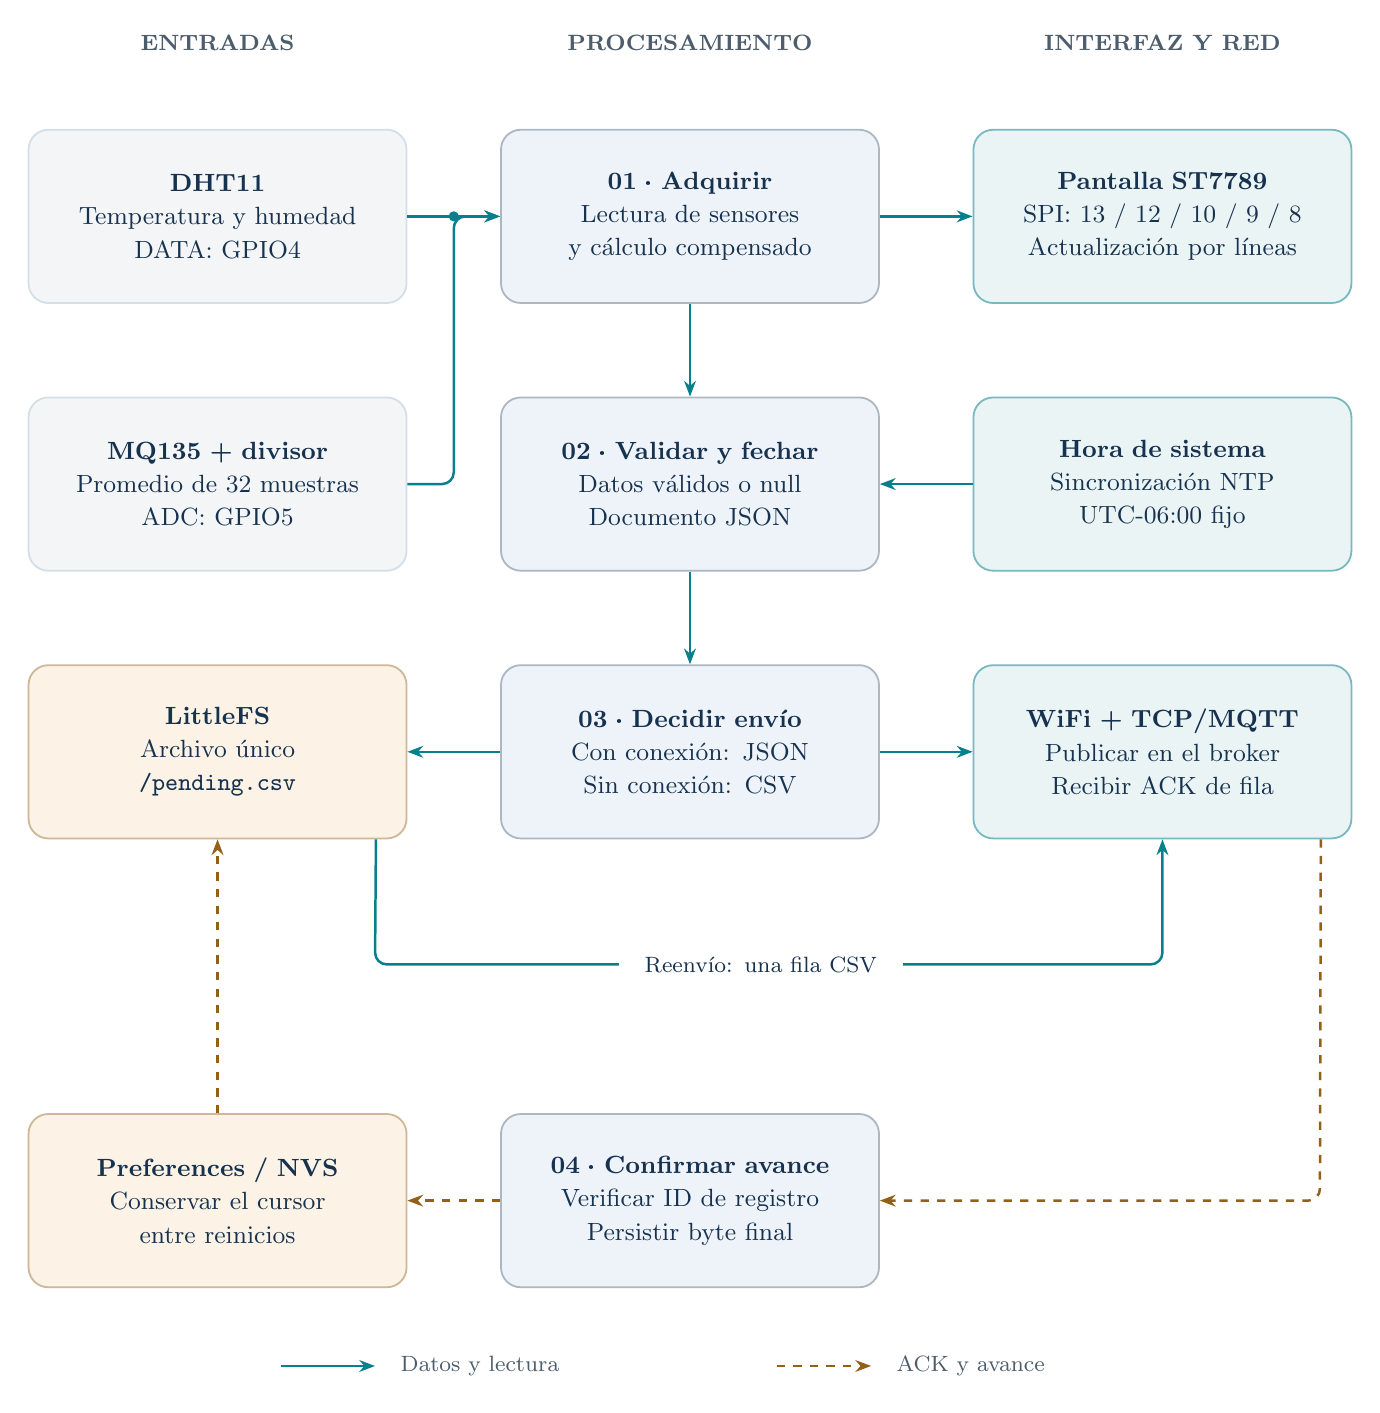
\begin{tikzpicture}[x=1mm,y=1mm]
\node[chip] at (25,0) {ENTRADAS};
\node[chip] at (85,0) {PROCESAMIENTO};
\node[chip] at (145,0) {INTERFAZ Y RED};

\node[card] (dht) at (25,-22) {\textbf{DHT11}\\Temperatura y humedad\\DATA: GPIO4};
\node[card] (mq) at (25,-56) {\textbf{MQ135 + divisor}\\Promedio de 32 muestras\\ADC: GPIO5};
\node[compute] (acq) at (85,-22) {\textbf{01 · Adquirir}\\Lectura de sensores\\y cálculo compensado};
\node[compute] (format) at (85,-56) {\textbf{02 · Validar y fechar}\\Datos válidos o null\\Documento JSON};
\node[compute] (route) at (85,-90) {\textbf{03 · Decidir envío}\\Con conexión: JSON\\Sin conexión: CSV};
\node[network] (tft) at (145,-22) {\textbf{Pantalla ST7789}\\SPI: 13 / 12 / 10 / 9 / 8\\Actualización por líneas};
\node[network] (ntp) at (145,-56) {\textbf{Hora de sistema}\\Sincronización NTP\\UTC-06:00 fijo};
\node[network] (mqtt) at (145,-90) {\textbf{WiFi + TCP/MQTT}\\Publicar en el broker\\Recibir ACK de fila};
\node[storage] (csv) at (25,-90) {\textbf{LittleFS}\\Archivo único\\\texttt{/pending.csv}};
\node[storage] (nvs) at (25,-147) {\textbf{Preferences / NVS}\\Conservar el cursor\\entre reinicios};
\node[compute] (ack) at (85,-147) {\textbf{04 · Confirmar avance}\\Verificar ID de registro\\Persistir byte final};

\draw[flow] (dht.east)--(acq.west);
\draw[flow] (mq.east)--(55,-56)--(55,-22)--(acq.west);
\fill[teal] (55,-22) circle (.65mm);
\draw[flow] (acq.south)--(format.north);
\draw[flow] (format.south)--(route.north);
\draw[flow] (acq.east)--(tft.west);
\draw[flow] (ntp.west)--(format.east);
\draw[flow] (route.west)--(csv.east);
\draw[flow] (route.east)--(mqtt.west);
% El historico utiliza su propio corredor, por debajo de la decision.
\draw[flow] ([xshift=-4mm]csv.south east)--(45,-117)--(145,-117)--(mqtt.south);
\node[message,text width=34mm,font=\fontsize{8}{10}\selectfont] at (94,-117) {Reenvío: una fila CSV};
% La confirmacion vuelve por un corredor distinto al del historico.
\draw[ackflow] ([xshift=-4mm]mqtt.south east)--(165,-147)--(ack.east);
\draw[ackflow] (ack.west)--(nvs.east);
\draw[ackflow] (nvs.north)--(csv.south);

\draw[flow] (33,-168)--(45,-168);
\node[anchor=west,font=\footnotesize,text=muted] at (47,-168) {Datos y lectura};
\draw[ackflow] (96,-168)--(108,-168);
\node[anchor=west,font=\footnotesize,text=muted] at (110,-168) {ACK y avance};
\end{tikzpicture}
\caption{Bloques del firmware y periféricos. Las flechas discontinuas indican confirmación o avance persistente.}
\end{figure}

\subsection{Organización interna}
\code{setup()} inicializa periféricos, archivos, NVS, WiFi, NTP y el cliente MQTT. \code{loop()} mantiene la conexión, atiende paquetes, agenda las lecturas y revisa el historial. El sketch no distribuye explícitamente sus funciones entre núcleos ni crea tareas propias de adquisición.

LittleFS conserva registros completos; NVS guarda un valor pequeño de avance. Es una separación apropiada entre archivos y pares clave--valor. Preferences conserva los datos entre reinicios.\cite{preferences} Ambos almacenamientos siguen siendo operaciones distintas, no una transacción indivisible.

\nextsection{Diagrama del sistema general y roles MQTT}
\begin{figure}[h!]
\centering
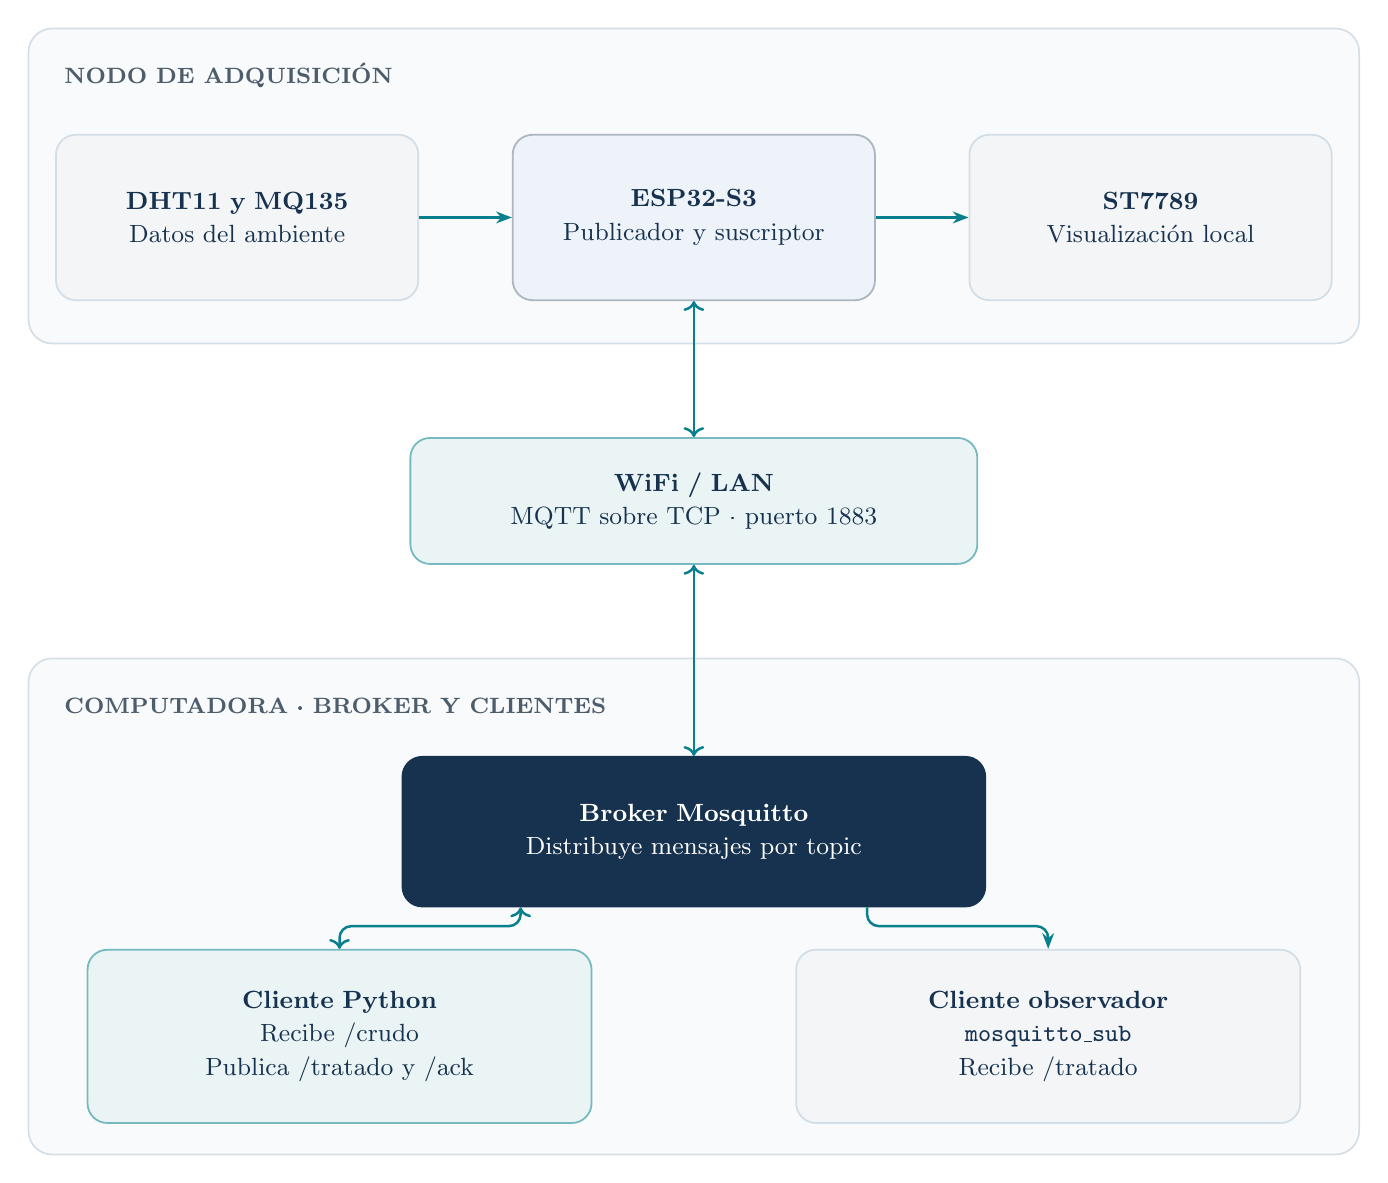
\begin{tikzpicture}[x=1mm,y=1mm]
% Agrupaciones fisicas: el nodo y la computadora son equipos diferentes.
\draw[groupbox] (.5,0) rectangle (169.5,-40);
\node[grouptitle] at (5,-6) {NODO DE ADQUISICIÓN};
\node[card,text width=40mm,minimum height=21mm] (sensors) at (27,-24)
  {\textbf{DHT11 y MQ135}\\Datos del ambiente};
\node[compute,text width=40mm,minimum height=21mm] (esp) at (85,-24)
  {\textbf{ESP32-S3}\\Publicador y suscriptor};
\node[card,text width=40mm,minimum height=21mm] (screen) at (143,-24)
  {\textbf{ST7789}\\Visualización local};
\draw[flow] (sensors.east)--(esp.west);
\draw[flow] (esp.east)--(screen.west);

\node[network,text width=66mm,minimum height=16mm,inner ysep=2mm] (lan) at (85,-60)
  {\textbf{WiFi / LAN}\\MQTT sobre TCP · puerto 1883};
\draw[flow,<->] (esp.south)--(lan.north);

\draw[groupbox] (.5,-80) rectangle (169.5,-143);
\node[grouptitle] at (5,-86) {COMPUTADORA · BROKER Y CLIENTES};
\node[strong,text width=68mm,minimum height=19mm,inner ysep=2mm] (broker) at (85,-102)
  {\textbf{Broker Mosquitto}\\Distribuye mensajes por topic};
\node[network,text width=58mm,minimum height=22mm,inner ysep=2mm] (python) at (40,-128)
  {\textbf{Cliente Python}\\Recibe /crudo\\Publica /tratado y /ack};
\node[card,text width=58mm,minimum height=22mm,inner ysep=2mm] (observer) at (130,-128)
  {\textbf{Cliente observador}\\\texttt{mosquitto\_sub}\\Recibe /tratado};
\draw[flow,<->] (lan.south)--(broker.north);
\draw[flow,<->] ([xshift=-22mm]broker.south)--(63,-114)--(40,-114)--(python.north);
\draw[flow] ([xshift=22mm]broker.south)--(107,-114)--(130,-114)--(observer.north);
\end{tikzpicture}
\caption{Sistema general: el broker intermedia; Python y ESP32 son clientes con roles de publicación y suscripción.}
\end{figure}

\begin{table}[h!]
\small
\begin{tabularx}{\linewidth}{@{}P{28mm}P{43mm}Y@{}}
\toprule
\textbf{Sufijo del topic} & \textbf{Publicador} & \textbf{Contenido y destinatario}\\\midrule
\code{/tratado} & ESP32 o Python & JSON uniforme; cliente observador y futuros consumidores.\\
\code{/crudo} & ESP32 & Cabecera CSV y una fila; Python escucha \code{dispositivo/+/crudo}.\\
\code{/ack} & Python & ID de la fila procesada; ESP32 escucha su topic específico.\\
\code{/estado} & ESP32 / broker & Conectado y Last Will desconectado; mensaje retenido.\\
\bottomrule
\end{tabularx}
\caption{Todos usan el prefijo \texttt{dispositivo/ESP32\_S3\_0001}. El signo + es comodín de suscripción.}
\end{table}

En la misma PC, Python puede conectarse a \code{127.0.0.1}. El ESP32 utiliza la IP LAN de la computadora; \code{0.0.0.0} en el listener significa escuchar interfaces IPv4, no una dirección que deba configurarse como broker remoto. Mosquitto se inicia como proceso separado del conversor.\cite{mosquitto}

\nextsection{Diagrama del proceso MQTT y confirmaciones}
\begin{figure}[h!]
\centering
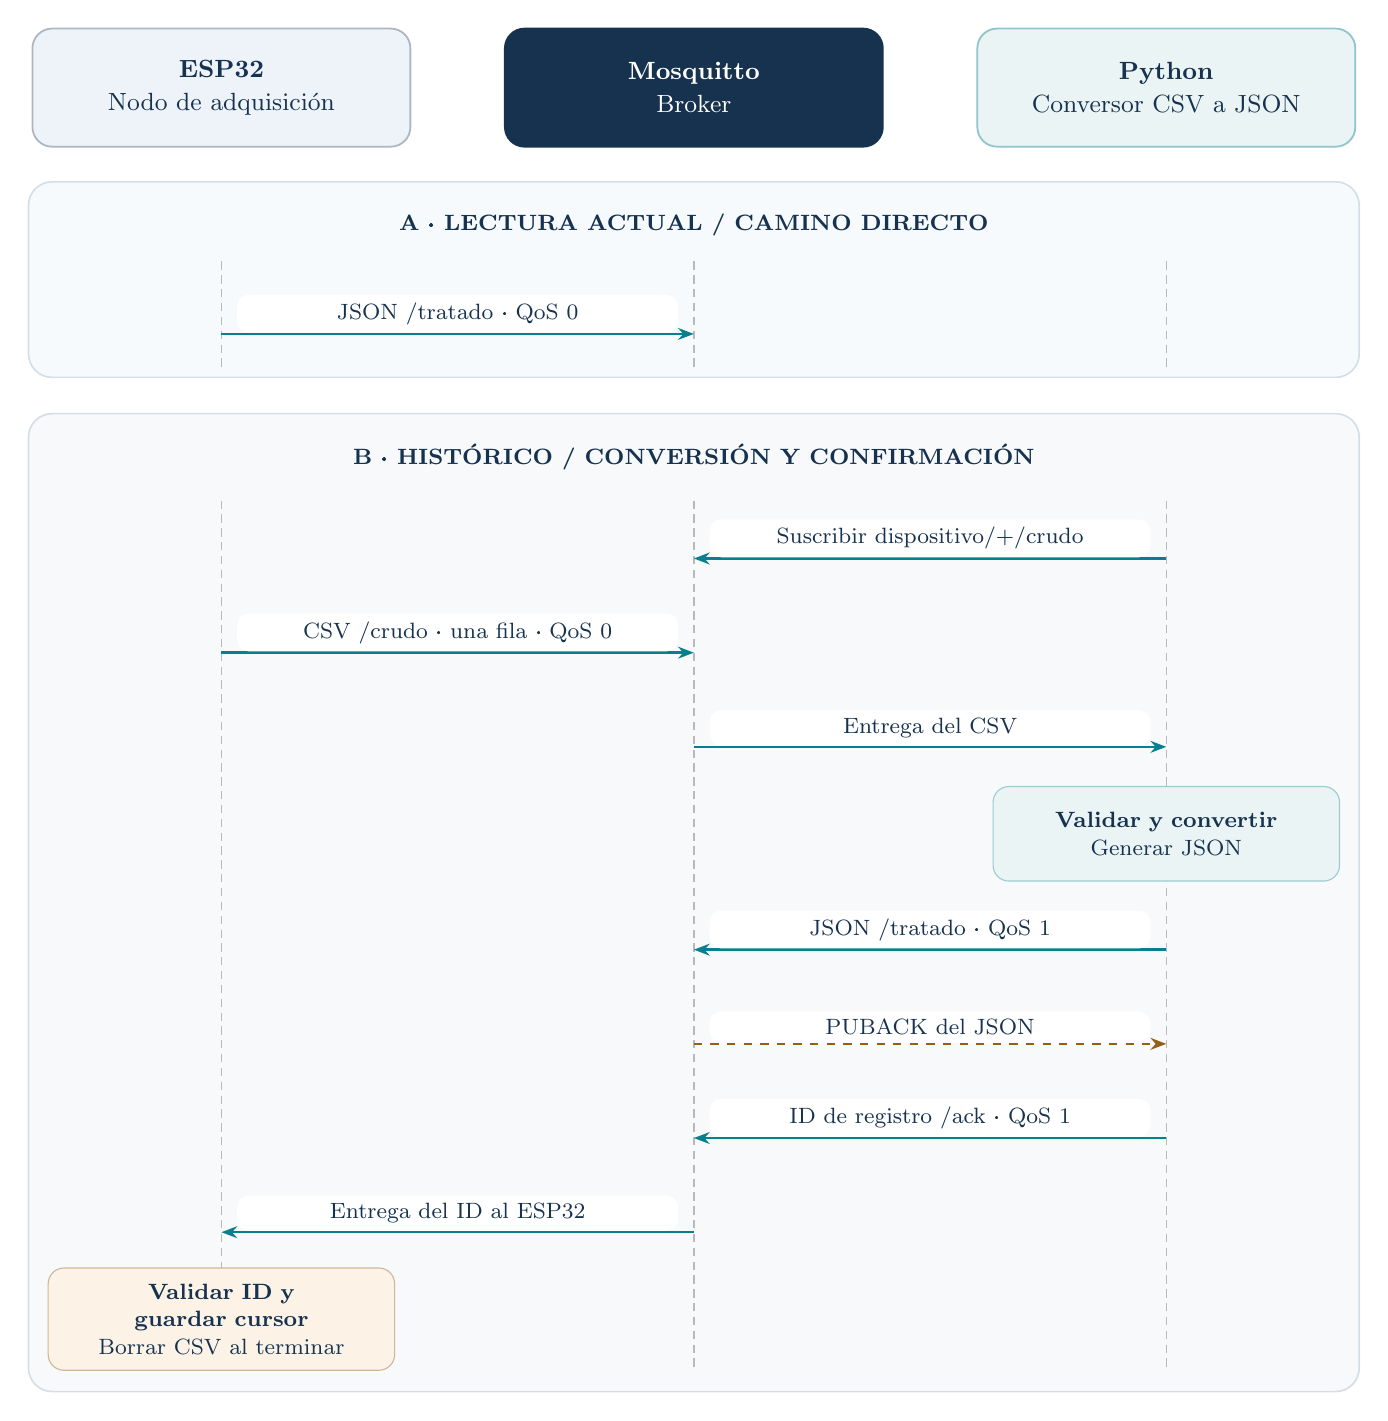
\begin{tikzpicture}[x=1mm,y=.92mm]
\node[participant,fill=bluepale,draw=navy!35] (esp) at (25,0) {\textbf{ESP32}\\Nodo de adquisición};
\node[participant,fill=navy,draw=navy,text=white] (broker) at (85,0) {\textbf{Mosquitto}\\Broker};
\node[participant,fill=pale,draw=teal!45] (python) at (145,0) {\textbf{Python}\\Conversor CSV a JSON};

\draw[groupbox,fill=bluepale!45] (.5,-13) rectangle (169.5,-40);
\draw[groupbox,fill=graybg!60] (.5,-45) rectangle (169.5,-180);
\node[chip,text width=145mm,text=navy] at (85,-19) {A · LECTURA ACTUAL / CAMINO DIRECTO};
\node[chip,text width=145mm,text=navy] at (85,-51) {B · HISTÓRICO / CONVERSIÓN Y CONFIRMACIÓN};

\foreach \x in {25,85,145} {
  \draw[gray!55,densely dashed,line width=.5pt] (\x,-24)--(\x,-39);
  \draw[gray!55,densely dashed,line width=.5pt] (\x,-57)--(\x,-177);
}
\draw[flow] (25,-34)--node[message,above]{JSON /tratado · QoS 0} (85,-34);

\draw[flow] (145,-65)--node[message,above]{Suscribir dispositivo/+/crudo} (85,-65);
\draw[flow] (25,-78)--node[message,above]{CSV /crudo · una fila · QoS 0} (85,-78);
\draw[flow] (85,-91)--node[message,above]{Entrega del CSV} (145,-91);
\node[activity] at (145,-103) {\textbf{Validar y convertir}\\Generar JSON};
\draw[flow] (145,-119)--node[message,above]{JSON /tratado · QoS 1} (85,-119);
\draw[ackflow] (85,-132)--node[message,above]{PUBACK del JSON} (145,-132);
\draw[flow] (145,-145)--node[message,above]{ID de registro /ack · QoS 1} (85,-145);
\draw[flow] (85,-158)--node[message,above]{Entrega del ID al ESP32} (25,-158);
\node[activity,text width=40mm,fill=warmpale,draw=amber!45] at (25,-170)
  {\textbf{Validar ID y guardar cursor}\\Borrar CSV al terminar};
\end{tikzpicture}
\caption{Secuencia simplificada. Se omiten CONNECT/CONNACK, SUBACK y parte de los intercambios de la publicación ACK para facilitar la lectura.}
\end{figure}

\subsection{Tres hechos diferentes}
El resultado verdadero de \code{PubSubClient.publish()} no prueba recepción del broker. El PUBACK que espera Python confirma la publicación MQTT del JSON; no prueba que un consumidor lo haya almacenado. El ACK de aplicación contiene el ID de la fila y permite avanzar el cursor solo si el firmware lo acepta y lo persiste.

La suscripción de Python solicita QoS 1, pero el crudo recibido desde ESP32 se publicó con QoS 0; la suscripción no eleva esa garantía. Si el JSON llega pero se pierde el ACK de aplicación, se repetirá la fila y puede duplicarse el JSON. No hay deduplicación en la implementación.

\nextsection{Adquisición, tratamiento y modelo del MQ135}
\subsection{DHT11, valores inválidos y hora}
\code{dhtSensor.readTemperature()} y \code{readHumidity()} entregan valores que el firmware valida con \code{isfinite()}. Una lectura no finita se representa como \code{null} en JSON y campo vacío en CSV. No se reemplaza por cero, porque cero sería un valor numérico con otro significado.

El MQ135 depende de temperatura y humedad válidas para su compensación. Por eso los tres valores pueden aparecer como \code{null} si falla el DHT11, sin que eso demuestre una avería del sensor de gas. Antes de reunir 30 muestras válidas de referencia también se devuelve \code{NAN} para gas.

NTP ajusta la hora de sistema. \code{getCurrentTimestamp()} produce una cadena ISO 8601 con UTC$-$06:00 fijo si el tiempo supera un umbral de plausibilidad; antes devuelve texto vacío. No se reconstruyen retrospectivamente fechas que faltaban al guardar una lectura. NTP y la referencia del gas son procesos independientes.

\subsection{Promedio ADC y reconstrucción eléctrica}
\code{analogReadMilliVolts()} obtiene el voltaje convertido a milivoltios según la API de Arduino-ESP32.\cite{adc} El programa toma 32 muestras con separaciones de 2 ms y calcula:
\[
V_{ADC}=\frac{\sum_{i=1}^{32} mV_i}{32\cdot1000},\qquad
V_{AO}=2V_{ADC}.
\]
Con dos resistencias de 10 k$\Omega$, el divisor reduce AO a la mitad. El modelo usa una carga de 2 k$\Omega$ en paralelo con la rama de 20 k$\Omega$:
\[
R_{L,ef}=\frac{2\cdot20}{2+20}\approx1.818\;\text{k}\Omega.
\]
La lectura se rechaza si $V_{ADC}<0.15$ V, $V_{ADC}\ge3$ V o $V_{AO}\ge5$ V. Son criterios del cálculo; no son una protección eléctrica.

\subsection{Compensación y referencia supuesta}
Para temperatura $T$ en °C y humedad $H$ en \%RH, el código aplica:
\[
f(T,H)=0.00035T^2-0.02718T+1.39538-0.0018(H-33),
\]
\[
R_{s,c}=\frac{(5/V_{AO}-1)R_{L,ef}}{f(T,H)}.
\]
Después de 30 muestras válidas estima la referencia $R_0$ suponiendo 450 ppm:
\[
R_0=\frac{\overline{R_{s,c}}}{(450/A)^{1/B}},\qquad
ppm=A\left(\frac{R_{s,c}}{R_0}\right)^B,
\quad A=110.47,\;B=-2.862.
\]
\note{Estas ecuaciones describen la implementación; no validan su exactitud física. El MQ135 responde a varios gases, el ambiente de referencia no se midió y $R_0$ se recalcula en cada arranque. Valores cercanos a 450 después de referenciar son esperables por construcción. \code{calibrate=false} permanece fijo; no cambia a true al completar las muestras.}

\nextsection{Aspectos relevantes del firmware C++}
\subsection{Bibliotecas y objetos}
\begin{table}[h!]
\small
\begin{tabularx}{\linewidth}{@{}P{39mm}Y@{}}
\toprule
\textbf{Biblioteca / objeto} & \textbf{Responsabilidad en la práctica}\\\midrule
Arduino / Serial, String & GPIO, tiempos, texto y diagnóstico a 115200 baudios.\\
DHT / dhtSensor & Lectura digital de temperatura y humedad en GPIO4.\\
TFT\_eSPI / display & Inicialización y dibujo en ST7789 con configuración propia.\\
WiFi / wifiClient & Asociación a la red y transporte TCP para el cliente MQTT.\\
PubSubClient / mqttClient & Conexión, publicación, suscripción y callback de ACK.\\
ArduinoJson / configuration & Carga de configuración y generación/serialización de JSON.\\
LittleFS / File & Archivo de configuración y cola CSV en flash.\\
Preferences / queuePreferences & Cursor confirmado de 32 bits en NVS.\\
math.h y time.h & Validación numérica, potencia, hora de sistema y formato de fecha.\\
\bottomrule
\end{tabularx}
\caption{Dependencias del firmware y sus responsabilidades.}
\end{table}

\subsection{Constantes y temporización}
Los GPIO se expresan con \code{constexpr uint8_t}; tiempos con \code{unsigned long}; posiciones de archivo con \code{size_t}; cálculos con \code{float}. \code{constexpr} exige un inicializador constante de compilación, mientras \code{const} prohíbe modificar el objeto mediante ese nombre aunque el valor se obtenga al ejecutar.
\begin{lstlisting}[language=C++]
constexpr unsigned long SAMPLE_INTERVAL_MS = 2000;
const float temperature = dhtSensor.readTemperature();
if (millis() - lastSampleAt >= SAMPLE_INTERVAL_MS) {
    lastSampleAt = millis();
    sampleAndPublish();
}
\end{lstlisting}
La resta sin signo mide tiempo transcurrido y evita comparar directamente marcas absolutas alrededor del desbordamiento de \code{millis()}. El diseño no es tiempo real estricto: red, sensores y flash consumen tiempo y algunas llamadas bloquean. Las lecturas se programan cada 2000 ms; reconexión y reenvío, cada 5000 ms. El buffer MQTT es 1024 bytes y el timeout de socket, 1 s.

Los prototipos se mantienen antes de \code{setup()} y las definiciones propias debajo de \code{loop()}. Nombres descriptivos, llaves explícitas y formato de cuatro espacios reducen ambigüedad al leer condiciones y rutas de error.

\clearpage
\subsection{Funciones y decisiones principales}
\begin{table}[h!]
\small
\begin{tabularx}{\linewidth}{@{}P{44mm}Y@{}}
\toprule
\textbf{Función} & \textbf{Contrato y efecto relevante}\\\midrule
\code{setup()} & Sin parámetros. Inicializa pantalla, LittleFS sin formatear, configuración, NVS, DHT/ADC, WiFi, NTP y MQTT. Si falla una condición requerida, no activa el sistema.\\
\code{loop()} & Sin parámetros. Atiende conexión y paquetes; agenda lectura y recuperación de historial.\\
\code{loadConfiguration()} & Devuelve bool. Deserializa archivo y valida SSID, PASS y MQTT\_HOST como texto.\\
\code{maintainMqttConnection()} & Sin parámetros. Reintenta WiFi/MQTT, registra transiciones y configura Last Will retenido.\\
\code{onMqttMessage(topic,payload,length)} & Recibe bytes del ACK; exige ID pendiente y guarda el byte final de fila en NVS.\\
\code{sampleAndPublish()} & Lee sensores, obtiene hora, serializa JSON y guarda CSV si no puede publicar.\\
\code{readGasPpm(T,H)} & Devuelve ppm estimadas o NAN; incorpora promedio, compensación y referencia.\\
\code{buildMeasurementJson(doc,ts,T,H,gas)} & Llena el documento recibido por referencia y preserva el esquema.\\
\code{updateDisplay(T,H,gas)} & Dibuja solamente las líneas cambiadas sobre fondo negro.\\
\code{saveMeasurementCsv(ts,T,H,gas)} & Agrega una fila al archivo único, con ID aleatorio.\\
\code{publishPendingCsv()} & Envía la primera fila pendiente o elimina el archivo si terminó.\\
\code{getCurrentTimestamp()} & Devuelve fecha local con desplazamiento fijo o cadena vacía.\\
\code{formatCsvNumber(value)} & Devuelve dos decimales o vacío si no es finito.\\
\bottomrule
\end{tabularx}
\caption{Síntesis funcional del código principal.}
\end{table}

\subsection{Interfaz local y diagnóstico}
El fondo se limpia por completo solo al iniciar. \code{updateDisplay()} conserva \code{previousLines} como variable estática, compara cada cadena y usa \code{setTextPadding(display.width())} para cubrir restos de texto anterior. Esto reduce redibujado, pero no garantiza eliminar cualquier artefacto físico o del controlador.

El mensaje ``Inicialización TFT terminada'' indica que regresó la llamada de biblioteca. No prueba que el panel haya recibido correctamente cada dato: no hay MISO para leer una respuesta del módulo. Un destello de fondo blanco debe investigarse por separado del parpadeo de letras.

\nextsection{Contrato JSON, CSV único y persistencia}
\subsection{Esquema uniforme}
Las lecturas actuales y las recuperadas llegan a \code{dispositivo/ESP32_S3_0001/tratado} con la misma estructura. Los espacios de serialización pueden diferir entre ArduinoJson y Python sin cambiar el significado.
\begin{lstlisting}
{
  "device_id": "ESP32_S3_0001",
  "timestamp": "2026-11-09T00:30:00-06:00",
  "measurements": {
    "temperature": {"sensor": "DHT11", "value": 23.4,
                    "unit": "\u00b0C"},
    "humidity": {"sensor": "DHT11", "value": 53,
                 "unit": "%RH"},
    "gas": {"sensor": "MQ135", "value": 452.7,
            "unit": "ppm", "calibrate": false}
  }
}
\end{lstlisting}
Es un ejemplo representativo, no una muestra nueva. \code{\u00b0C} representa el mismo símbolo °C en JSON. Las fechas desconocidas y los valores inválidos se expresan como \code{null}; no se elimina la clave ni se simula una lectura.

\subsection{Una fila, una confirmación}
La cabecera es \code{id,device_id,timestamp,temperature,humidity,gas,calibrate}. Un archivo puede contener muchas filas; el mensaje crudo incluye solo cabecera y la fila que se está intentando confirmar. El ID del registro se forma con dos valores aleatorios hexadecimales. Ese ID no es el ID del dispositivo ni aparece en el JSON final.

En NVS, el espacio \code{csv-queue} y la clave \code{offset} guardan el cursor. Por ejemplo, si la cabecera ocupa $H$ bytes y la primera fila $A$, el primer ACK persistido deja el cursor en $H+A$. Un reinicio puede recuperar esa posición y continuar con la siguiente fila. Solo se avanza si coinciden los IDs y \code{putULong()} informa la cantidad esperada de bytes.

\subsection{Borrado y límites del historial}
Las filas confirmadas permanecen dentro del archivo hasta terminar el historial. En una revisión posterior, si el cursor alcanza su tamaño, se elimina \code{/pending.csv}. Si se añadieron filas, también deben confirmarse. Con menos de 8192 bytes libres se rechaza una nueva escritura y se informa por Serial.

Una escritura parcial puede dejar una fila que Python rechace indefinidamente. CSV y cursor NVS no se actualizan atómicamente. Cargar \code{uploadfs} puede reemplazar archivos sin reiniciar el cursor NVS; no debe usarse sobre una cola activa sin gestionar ese estado. La implementación no promete tolerancia total a cortes de energía.

\nextsection{Modularización del cliente Python}
\begin{table}[h!]
\small
\begin{tabularx}{\linewidth}{@{}P{41mm}Y@{}}
\toprule
\textbf{Archivo} & \textbf{Responsabilidad}\\\midrule
\code{scripts/csv_to_json.py} & Entrada ejecutable: selecciona el import y llama a main.\\
\code{mqtt_bridge/settings.py} & Filtro de topic, cola, tiempos y contrato de campos/unidades.\\
\code{mqtt_bridge/models.py} & Dataclass ConvertedReading: device\_id, record\_id y json\_payload; campos frozen.\\
\code{mqtt_bridge/converter.py} & Valida topic/UTF-8/CSV, transforma números y construye JSON sin red.\\
\code{mqtt_bridge/bridge.py} & Callbacks, cola, trabajador, publicación tratada y ACK.\\
\code{mqtt_bridge/cli.py} & Argumentos --host/--port, cliente Paho y ciclo MQTT.\\
\code{mqtt_bridge/__init__.py} & Identidad del paquete, sin arranque de conexiones.\\
\bottomrule
\end{tabularx}
\caption{Separación de responsabilidades del programa Python.}
\end{table}

\subsection{Conversión y validación}
\code{convert_csv_message(topic,payload)} exige un topic de tres niveles, cabecera exacta y una sola fila con siete campos. Comprueba coincidencia de dispositivo, ID de registro no vacío y \code{calibrate} textual válido. \code{parse_measurement()} devuelve \code{None} ante vacío, un \code{float} finito ante un número y error ante dato no válido. \code{json.dumps(...,allow_nan=False)} evita generar NaN/Infinity no estándar.

El conversor devuelve \code{ConvertedReading}, separando identificación para confirmar de contenido JSON. No crea clientes ni lee archivos de configuración. Esa independencia permite probar reglas de datos sin disponer del broker.

\subsection{Cola, callbacks e hilos}
\code{on_message()} encola \code{(topic,payload)} sin esperar espacio. La cola admite 100 elementos. El trabajador ejecuta conversión y publicación; espera hasta 10 s para verificar \code{is_published()}. Mientras espera, el hilo de red debe seguir recibiendo paquetes. Separarlos evita bloquear el procesamiento del PUBACK.\cite{paho}

Si la publicación está confirmada, \code{publish_reading()} envía el ID a \code{/ack}. Si no, conserva la fila en el ESP32 por ausencia de confirmación. \code{task_done()} solo cierra el trabajo local de la cola: no es un ACK MQTT. El hilo es daemon y no cuenta con vaciado garantizado al salir. El keepalive configurado para Python es 60 s.

\subsection{Imports y ejecución}
Los imports relativos como \code{from .models import ConvertedReading} mantienen dependencias dentro del paquete. La entrada admite ejecución directa o \code{python -m scripts.csv_to_json} desde la raíz. Los módulos no deben lanzarse aisladamente como sustitutos de esa entrada. La única dependencia externa declarada es \code{paho-mqtt>=2.1,<3}; modularizar no añadió un framework.

\nextsection{Procedimiento práctico de puesta en marcha}
\subsection{Firmware y archivos}
\begin{lstlisting}
# Desde la carpeta del proyecto
pio run
pio run -e esp32-s3-devkitc-1 -t upload
# Solo para cargar data/ y con cuidado del historial:
pio run -e esp32-s3-devkitc-1 -t uploadfs
\end{lstlisting}
\textbf{Build} compila; \textbf{Upload} compila y escribe el firmware; \textbf{Upload Filesystem Image} carga archivos. La pestaña abierta no selecciona el código: el entorno principal filtra \code{main.cpp}, mientras los entornos de prueba seleccionan \code{display_test.cpp}.

\subsection{Broker y cliente}
\begin{lstlisting}
# Terminal 1: broker (mantener abierto)
mosquitto -c scripts/mosquitto.conf -v

# Terminal 2: conversor, usando el entorno instalado
.venv/bin/python scripts/csv_to_json.py --host 127.0.0.1

# Terminal 3: observacion de JSON
mosquitto_sub -h 127.0.0.1 -p 1883 \
  -t 'dispositivo/+/tratado' -v
\end{lstlisting}
\begin{lstlisting}
# scripts/mosquitto.conf
listener 1883 0.0.0.0
allow_anonymous true
\end{lstlisting}
En \code{data/config.json}, \code{MQTT_HOST} debe ser la IP LAN de la computadora y \code{MQTT_PORT} un número, habitualmente 1883. \code{SSID} y \code{PASS} corresponden al WiFi, no a autenticación MQTT. Esta práctica conecta anónimamente y sin TLS; no establece controles de producción.\cite{mosquitto}

Si aparece ``Address already in use'', se verifica el proceso que ocupa el puerto antes de iniciar otra instancia. La ruta del archivo de configuración es relativa al directorio de trabajo. Ante \code{ModuleNotFoundError: paho}, se utiliza el Python de \code{.venv} y se instala \code{scripts/requirements.txt} si hace falta.

\subsection{Prueba de desconexión}
Se observan primero lecturas directas. Se interrumpe temporalmente el broker, se espera a que se generen registros y se restablece. El ESP32 debe reenviar filas, Python tratarlas y el dispositivo avanzar con sus ACK. Una cola grande tarda en vaciarse: el ritmo nominal de recuperación es 0.2 filas/s frente a 0.5 muestras/s durante adquisición. Las lecturas actuales que se publican bien no vuelven a anexarse al CSV al reconectar.

\nextsection{Resultados observados y validación}
La tabla reúne evidencia de terminales y capturas compartidas, junto con revisión de lógica y ejercicios offline. No presenta promedios estadísticos, porcentajes de error ni autonomía que no se hayan medido.

\begin{table}[h!]
\footnotesize
\begin{tabularx}{\linewidth}{@{}P{26mm}P{49mm}Y@{}}
\toprule
\textbf{Aspecto} & \textbf{Resultado / evidencia} & \textbf{Interpretación y alcance}\\\midrule
Compilación y carga & Registros de compilación y verificación de hash exitosos para main.cpp. & Demuestra construcción y carga, no precisión del montaje.\\
MQTT directo & Broker recibe /tratado del ESP32 aproximadamente cada 2 s. & Se verificó el camino de lecturas actuales.\\
Temperatura & Valores observados de 23 a 23.4 °C. & DHT entrega números válidos; no hubo comparación contra termómetro patrón.\\
Humedad & Valores observados de 53 a 54 \%RH. & Se comprobó publicación del dato; no se midió exactitud.\\
Gas estimado & Pasó de null a valores numéricos; ejemplos de aproximadamente 413 a 460 ppm. & Se completó referencia y cálculo. Cercanía a 450 no valida concentración real.\\
Fecha/hora & Timestamp pasó de null a fecha con $-$06:00. & Evidencia de hora disponible; no se midió su error temporal.\\
Conversión Python & /crudo recibido, seguido de /tratado QoS 1 y PUBACK en logs. & Se verificó tratamiento y publicación del historial.\\
ACK y avance & ACK entregados al ESP32; fechas históricas sucesivas. & Evidencia de confirmación y progreso. Un PUBACK no prueba por sí solo escritura NVS.\\
Borrado CSV & Se aportaron mensajes Serial ``CSV confirmado y eliminado''. & Evidencia de la ruta de borrado en esas ejecuciones; no se inspeccionó toda la flash.\\
Pantalla & Usuario confirmó visualización de temperatura, humedad y ppm. & Funcionalidad básica observada; destello blanco posterior pendiente.\\
Lógica modular & Ejercicios offline de conversión, rechazo, cola, ACK y CLI ejecutados sin broker. & Validan decisiones de software, no transporte físico ni persistencia del ESP32.\\
Calidad metrológica & Sin medición contra referencia ni ensayo controlado de gas. & Precisión, selectividad y error absoluto permanecen sin determinar.\\
\bottomrule
\end{tabularx}
\caption{Tabla de resultados y límites de interpretación. Los rangos son ejemplos de fragmentos aportados, no un estudio estadístico.}
\end{table}

\subsection{Lecturas actuales e históricas intercaladas}
Se observaron documentos con horas actuales intercalados con fechas anteriores que avanzaban de forma sucesiva. Ese comportamiento corresponde al diseño: las lecturas en vivo van directamente a \code{/tratado} mientras Python publica el historial. No existe orden cronológico global entre ambos publicadores; un consumidor que lo requiera debe ordenar por timestamp y tratar fechas nulas.

\nextsection{Incidencias, diagnóstico y aprendizajes prácticos}
\begin{table}[h!]
\small
\begin{tabularx}{\linewidth}{@{}P{38mm}YY@{}}
\toprule
\textbf{Incidencia} & \textbf{Acción y hallazgo} & \textbf{Aprendizaje}\\\midrule
Puerto 1883 ocupado & Se identificó Mosquitto ya escuchando como servicio antes de ejecutar otra instancia. & Un mismo puerto no puede asignarse de esa forma a dos listeners simultáneos.\\
Archivo de broker no encontrado & Se corrigió el directorio desde el que se ejecutaba la ruta scripts/mosquitto.conf. & Las rutas relativas dependen del directorio de trabajo.\\
Paho ausente al ejecutar & Se verificó .venv: Paho estaba instalado; faltaba usar el intérprete correcto. & Instalar en un entorno no habilita otro Python distinto.\\
Valores null & DHT y gas comenzaron inválidos; después aparecieron valores. & Distinguir ausencia de lectura, referencia en curso y cero físico.\\
Pantalla y entorno activo & Se aclaró que Upload había cargado main, aunque estaba abierta la prueba. & PlatformIO elige fuentes por entorno, no por pestaña.\\
Causalidad de FSPI/5 MHz & El usuario confirmó imagen antes del último ajuste; el principal volvió a HSPI/20 MHz. & No atribuir una mejora a cambios que ocurrieron después del resultado.\\
Destello blanco & Se revisaron conexiones y se prepararon variantes aisladas. No se confirmó causa. & Separar redibujado, reinicios, alimentación, controlador y señal SPI con pruebas.\\
\bottomrule
\end{tabularx}
\caption{Incidencias relevantes y conocimiento obtenido.}
\end{table}

\subsection{Pantalla: condición aún abierta}
El usuario reportó destellos de fondo blanco. El firmware normal dibuja sobre fondo negro y evita limpiar toda la pantalla en cada lectura; el firmware de prueba alterna colores deliberadamente. Para investigar se requiere identificar el entorno realmente cargado, correlacionar el destello con Serial y medir estabilidad eléctrica. La alimentación declarada de 3.3 V no demuestra por sí sola la causa.

Los registros con arranques POWERON y advertencia de checksum de core dump no establecen una causa única del problema. El core dump corresponde a información de diagnóstico guardada.\cite{coredump} No se debe borrar toda la flash ni modificar tensiones como respuesta automática a ese mensaje.

\subsection{Calidad del código}
La práctica incorporó nombres descriptivos, constantes con unidades, validaciones tempranas, prototipos ordenados, indentación consistente y separación modular. La documentación secuencial en notebooks conserva explicaciones y ejercicios, y su carpeta está excluida de Git según el alcance solicitado. El reporte resume lo más relevante sin sustituir el código fuente ni los notebooks detallados.

\nextsection{Ventajas y desventajas de la implementación}
\subsection{Ventajas}
\begin{table}[h!]
\small
\begin{tabularx}{\linewidth}{@{}P{40mm}Y@{}}
\toprule
\textbf{Ventaja} & \textbf{Beneficio concreto}\\\midrule
Visualización local & Lecturas disponibles en el nodo sin depender de que un consumidor de PC esté abierto.\\
Formato JSON uniforme & Un consumidor recibe el mismo esquema para datos actuales e históricos.\\
Historial persistente & Las filas pueden sobrevivir una desconexión y reanudarse con un cursor NVS.\\
Confirmación de aplicación & No se retira una fila del conjunto pendiente solo por intentar enviarla.\\
Topics por dispositivo & El filtro + permite ampliar a varios IDs sin añadir una suscripción por nodo.\\
Modularidad y pruebas & El conversor puede verificarse sin crear un broker ni conectar hardware.\\
Configuración reproducible & Pines TFT fuera de .pio y dependencias declaradas en PlatformIO.\\
Operación local & Broker y conversor funcionan dentro de la LAN; no requieren un servicio MQTT de nube.\\
\bottomrule
\end{tabularx}
\end{table}

\subsection{Desventajas y compromisos}
\begin{table}[h!]
\small
\begin{tabularx}{\linewidth}{@{}P{40mm}Y@{}}
\toprule
\textbf{Límite} & \textbf{Consecuencia práctica}\\\midrule
QoS 0 en ESP32 & Una publicación actual que devuelve verdadero todavía puede perderse sin entrar al CSV.\\
Duplicados e intercalado & ACK perdido puede repetir JSON; datos actuales e históricos no llegan globalmente ordenados.\\
Capacidad flash finita & Con poco espacio se descartan nuevas filas; no hay almacenamiento ilimitado ni rotación automática.\\
Fallo parcial de escritura & Una fila incompleta puede detener el vaciado; no existe reparación automática.\\
MQ135 no contrastado & Ppm son estimadas con referencia supuesta; no aptas para certificar CO\textsubscript{2}.\\
Seguridad de laboratorio & MQTT anónimo y sin TLS carece de autenticación y cifrado de aplicación en la configuración usada.\\
Operación no determinista & Lecturas, flash y conexión bloquean parcialmente loop; recuperación limitada a una fila cada 5 s.\\
Dependencia operativa & Python y broker deben estar activos para tratar históricos; error inicial de conexión Python no tiene reintento propio.\\
\bottomrule
\end{tabularx}
\end{table}

\nextsection{Conclusiones y mejoras propuestas}
La práctica integró adquisición, visualización, mensajería y persistencia en un sistema funcional. Los registros verifican que el ESP32 publica mediciones actuales y que el conversor procesa filas históricas, publica JSON y envía confirmaciones. La modularización mantuvo el protocolo y permitió comprobar reglas del conversor sin infraestructura de red.

El diseño demuestra recuperación controlada de un historial, pero no entrega exactamente una vez ni continuidad metrológica garantizada. El MQ135 produce una estimación condicionada por el ambiente supuesto y la compensación. La pantalla mostró mediciones, aunque el destello blanco reportado sigue pendiente de diagnóstico. No se concluye que cambiar a FSPI o reducir frecuencia haya resuelto ese síntoma.

\subsection{Mejoras posteriores, no implementadas}
\begin{enumerate}
\setlength\itemsep{2pt}
\item \textbf{Calidad de medición:} estabilizar el MQ135 según su módulo, caracterizarlo en condiciones conocidas y contrastar con instrumento de referencia. Registrar R0 y condiciones de calibración cuando exista una calibración real.
\item \textbf{Integridad de datos:} incluir un identificador de muestra en el JSON final, deduplicar consumidores y estudiar un cliente ESP32 con QoS de publicación confirmado cuando la pérdida no sea aceptable.
\item \textbf{Persistencia:} detectar o aislar filas corruptas, coordinar cursor y archivo ante cortes, controlar desgaste y gestionar explícitamente el reemplazo de LittleFS.
\item \textbf{Operación:} añadir reconexión inicial Python, apagado ordenado del trabajador, métricas de cola pendiente y política de recuperación que no bloquee el muestreo.
\item \textbf{Red y acceso:} para un despliegue fuera de laboratorio, definir autenticación, autorización por topic y TLS con gestión de certificados.
\item \textbf{Pantalla:} registrar reinicios, medir alimentación y señales; comparar configuraciones de una variable a la vez antes de atribuir causalidad al código o voltaje.
\end{enumerate}

\subsection{Evidencia y reproducibilidad}
La base local del reporte es el firmware principal, \code{platformio.ini}, \code{include/TFT_Setup.h}, la configuración anónima de Mosquitto y el paquete \code{scripts/mqtt_bridge/}. La evidencia experimental procede de capturas y logs compartidos durante la práctica del 8--9 de noviembre de 2026. No se ejecutaron nuevas cargas de firmware ni cambios de cableado para redactar este documento.

El código completo permanece en el proyecto; \code{docs/notebooks/} amplía teoría, funciones y ejercicios. El archivo \code{reporte_monitor_aire.tex} acompaña al PDF como fuente editable. Los diagramas son vectoriales y representan la configuración principal vigente: HSPI a 20 MHz, pantalla MOSI13, DHT4 y ADC5.

\clearpage
\begin{thebibliography}{9}
\small
\bibitem{mqtt} OASIS. \emph{MQTT Version 3.1.1}. Modelo de publicación/suscripción y QoS. \url{https://docs.oasis-open.org/mqtt/mqtt/v3.1.1/mqtt-v3.1.1.html}. Consulta: 9 de noviembre de 2026.
\bibitem{rfc1122} R. Braden, ed. \emph{RFC 1122: Requirements for Internet Hosts -- Communication Layers}. IETF, 1989. \url{https://www.rfc-editor.org/rfc/rfc1122.html}.
\bibitem{adc} Espressif Systems. \emph{Arduino-ESP32: ADC API}. \url{https://docs.espressif.com/projects/arduino-esp32/en/latest/api/adc.html}. Consulta: 9 de noviembre de 2026.
\bibitem{preferences} Espressif Systems. \emph{Arduino-ESP32: Preferences API}. \url{https://docs.espressif.com/projects/arduino-esp32/en/latest/api/preferences.html}. Consulta: 9 de noviembre de 2026.
\bibitem{mosquitto} Eclipse Mosquitto. \emph{mosquitto.conf man page}. Listeners y acceso anónimo. \url{https://mosquitto.org/man/mosquitto-conf-5.html}. Consulta: 9 de noviembre de 2026.
\bibitem{paho} Eclipse Paho. \emph{Python MQTT client module}. Callbacks, bucle de red y estado de publicación. \url{https://eclipse.dev/paho/files/paho.mqtt.python/html/client.html}. Consulta: 9 de noviembre de 2026.
\bibitem{coredump} Espressif Systems. \emph{ESP-IDF: Core Dump, ESP32-S3}. \url{https://docs.espressif.com/projects/esp-idf/en/stable/esp32s3/api-guides/core_dump.html}. Consulta: 9 de noviembre de 2026.
\end{thebibliography}

\subsection*{Fuentes primarias de la implementación}
\begin{itemize}
\item \code{src/main.cpp} y \code{src/display_test.cpp}.
\item \code{platformio.ini} e \code{include/TFT_Setup.h}.
\item \code{scripts/csv_to_json.py}, \code{scripts/mqtt_bridge/*.py} y \code{scripts/requirements.txt}.
\item \code{scripts/mosquitto.conf}, \code{docs/pending.example.csv} y \code{README.md}.
\item Registros de carga, mensajes MQTT y observaciones físicas aportadas por el usuario.
\end{itemize}
\vfill
\noindent\rule{\linewidth}{0.4pt}\par
{\small\color{muted}Fin del reporte. Las observaciones describen esta implementación y su evidencia disponible; no sustituyen una certificación del instrumento ni una evaluación eléctrica del montaje.}
\end{document}
